% Initial version by Darian Muresan, Ph.D.
% Edit and adjust as needed.

\documentclass[12pt]{cornell}

% add index support
\makeindex

% graphing programs
\usepackage{color}
\usepackage{psfrag}
\usepackage{verbatim}
\usepackage{fancyhdr}
%\usepackage{titlesec}
\usepackage{fancyvrb} 
% hyperlink programs
\usepackage[pdfmark, 
breaklinks=true, 
colorlinks=true,
citecolor=blue,
linkcolor=blue,
menucolor=black,
pagecolor=black,
urlcolor=blue
]{hyperref} % links in pdf
%\usepackage[colorlinks]{hyperref} % links in dvi
\usepackage{listings}
\usepackage{amsfonts} 
\usepackage{amssymb} 
%\usepackage{tabto}

\usepackage{tabularx,colortbl}
\usepackage[chapter]{algorithm} 
\usepackage{algorithmic} 
\usepackage{blindtext}
\usepackage{imakeidx}


\definecolor{DarkGreen}{rgb}{0,0.6,0}
\definecolor{mygreen}{rgb}{0,0.6,0}
\definecolor{mygray}{rgb}{0.5,0.5,0.5}
\definecolor{mymauve}{rgb}{0.58,0,0.82}

\usepackage{tocloft}
\usepackage{amsmath}
\usepackage{tcolorbox}
\usepackage{enumitem}
\usepackage{longtable}
%\usepackage{textcomp}
\usepackage{txfonts}

%part for \part titles
%chap for \chapter titles
%sec for \section titles
%subsec for \subsection titles
%subsubsec for \subsubsection titles
%para for \paragraph titles
%subpara for \subparagraph titles
%fig for figure \caption titles
%subfig for subfigure \caption titles
%tab for table \caption titles
%subtab for subtable \caption titles

% update chapter number spacing
\setlength{\cftchapnumwidth}{2em}
\setlength{\cftsecnumwidth}{2.5em}
\setlength{\cftsubsecnumwidth}{3.5em}
\setlength{\cftsubsubsecnumwidth}{4.5em}

\addtolength{\cftsecindent}{0.5em}
\addtolength{\cftsubsecindent}{0.5em}
\addtolength{\cftsubsubsecindent}{0.5em}

%\titlespacing*{\chapter}{0pt}{-50pt}{20pt}
%\titleformat{\chapter}[display]{\normalfont\huge\bfseries}{\chaptertitlename\ 
%\thechapter}{20pt}{\Huge}
%\pagestyle{fancy}
%\pagestyle{cornell}
%
%\rhead{F054-021-0172}
%\chead{Nonlinear Enhancement of Visual Target Detection (AF05-T021)}
%\lhead{GSTI}
%\lfoot{\scriptsize Use or disclosure of data on this page is subject
%to the restriction on the title page of this proposal.}
%\cfoot{}
%\rfoot{\thepage}

\newfont{\Bp}{msbm10}
\newfont{\BpBig}{msbm10 scaled\magstep2}
\newfont{\Sc}{eusm10}
\newfont{\ScBig}{eusm10 scaled\magstep3}
\newfont{\Fr}{eufm10}
\newfont{\FrBig}{eufm10 scaled\magstep1}

% some commands:
\newcommand{\dxi}{{\tt m\_xDeltaInput}}
\newcommand{\dyi}{{\tt m\_yDeltaInput}}
\newcommand{\dci}{{\tt m\_cDeltaInput}}
\newcommand{\dxo}{{\tt m\_xDeltaOutput}}
\newcommand{\dyo}{{\tt m\_yDeltaOutput}}
\newcommand{\dco}{{\tt m\_cDeltaOutput}}
\newcommand{\ttf}[1]{{\tt #1}}
\newcommand{\tbl}[2]{{\begin{tabular}{c} #1 \\ #2 \end{tabular}}}

\newcommand{\urltwo}[2]{\mbox{\href{#1}{\tt #2}}}
\newcommand{\qnorm}[1]{\|#1\|_{\bQ}}
\newcommand{\qdot}[2]{\lrb #1, #2 \rrb_{\bQ}}
\newcommand{\kdot}[2]{\lrb #1, #2 \rrb_{\bf k}}
\newcommand{\tdot}[2]{\lrb #1, #2 \rrb}
\newcommand{\mydiff}[2]{\lrb #1 - #2 \rrb}
\newcommand{\lena}{\textit{lena}}
\newcommand{\barb}{\textit{barbara}}
\newcommand{\boat}{\textit{boat}}
\newcommand{\leaves}{\textit{leaves}}
\newcommand{\rings}{\textit{rings}}
\newcommand{\treg}{\textit{train region}}
\newcommand{\dreg}{\textit{denoise region}}
\newcommand{\oreg}{\textit{overlap region}}
\newcommand{\sil}{\sigma_l^2}
\newcommand{\sn}{\sigma^2}
\newcommand{\bn}{{\mbox{\bf \FrBig N}}}
\newcommand{\n}{\mbox{\Fr N}}
%\newcommand{\bn}{\bf N}
%\newcommand{\n}{N}
\newcommand{\bY}{\textbf{Y}}
\newcommand{\bX}{\textbf{X}}
\newcommand{\bb}{\textbf{b}}
\newcommand{\bu}{\textbf{u}}
\newcommand{\bv}{\textbf{v}}
\newcommand{\by}{\textbf{y}}
\newcommand{\bx}{\textbf{x}}
\newcommand{\be}{\textbf{e}}
\newcommand{\bz}{\textbf{z}}
\newcommand{\bs}{\textbf{s}}
\newcommand{\bw}{\textbf{w}}
\newcommand{\bQ}{\textbf{Q}}
\newcommand{\bphi}{\textbf{$\phi$}}
\newcommand{\lsb}{\left[}
\newcommand{\rsb}{\right]}
\newcommand{\lrb}{\left(}
\newcommand{\rrb}{\right)}
\newcommand{\lcb}{\left\{}
\newcommand{\rcb}{\right\}}
\newcommand{\R}{\mbox{\BpBig R}}
\newcommand{\F}{{\cal F}}
\newcommand{\Fk}{\mbox{\Sc F}}
\newcommand{\bQF}{\textbf{Q}_{\mbox{\Sc F}}}
\newcommand{\N}{{\cal N}}
\newcommand{\xlz}{X_l(z)}
\newcommand{\xhz}{X_h(z)}
\newcommand{\xz}{X(z)}
\newcommand{\pr}{ perfect reconstruction }
\newcommand{\smb}{Smith-Barnwell }
\newcommand{\xw}{X(e^{j\omega})}
\newcommand{\xmw}{X(-e^{j\omega})}
\newcommand{\dw}{D(e^{j\omega})}
\newcommand{\dmw}{D(-e^{j\omega})}
\newcommand{\ew}{E(e^{j\omega})}
\newcommand{\emw}{E(-e^{j\omega})}
\newcommand{\fw}{F_0(e^{j\omega})}
\newcommand{\fmw}{F_0(-e^{j\omega})}
\newcommand{\hoz}{H_1(z)}
\newcommand{\hzz}{H_0(z)}
\newcommand{\goz}{G_1(z)}
\newcommand{\gzz}{G_0(z)}
\newcommand{\hzw}{H_{0}(e^{j\omega})}
\newcommand{\hzmw}{H_{0}(-e^{j\omega})}
\newcommand{\hzcw}{H_{0}(e^{-j\omega})}
\newcommand{\how}{H_1(e^{j\omega})}
\newcommand{\homw}{H_1(-e^{j\omega})}
\newcommand{\gzw}{G_0(e^{j\omega})}
\newcommand{\gzmw}{G_0(-e^{j\omega})}
\newcommand{\gow}{G_1(e^{j\omega})}
\newcommand{\gomw}{G_1(-e^{j\omega})}
\newcommand{\wl}{e^{-jwL}}
\newcommand{\aqua}{\textit{AQua with OR }}
\newtheorem{theorem}{Theorem}
\newtheorem{lemma}{Lemma}
\newtheorem{corollary}{Corollary}
\newtheorem{claim}{Claim}
\newtheorem{definition}{Definition}
\newenvironment{proof}{\noindent{\em Proof.}}{\ \hfill Q.E.D.}
%\newtheorem{moduleCount}{L}
\newcommand*{\labelfile}[1]{%
  \label{file:#1}%
}

\lstset{ %
  backgroundcolor=\color{white},   % choose the background color; you must add \usepackage{color} or \usepackage{xcolor}
  basicstyle=\footnotesize,        % the size of the fonts that are used for the code
  breakatwhitespace=false,         % sets if automatic breaks should only happen at whitespace
  breaklines=true,                 % sets automatic line breaking
  captionpos=b,                    % sets the caption-position to bottom
  commentstyle=\color{DarkGreen},    % comment style
  deletekeywords={...},            % if you want to delete keywords from the given language
  escapeinside={\%*}{*)},          % if you want to add LaTeX within your code
  extendedchars=true,              % lets you use non-ASCII characters; for 8-bits encodings only, does not work with UTF-8
  %frame=single,                   % adds a frame around the code
  keepspaces=true,                 % keeps spaces in text, useful for keeping indentation of code (possibly needs columns=flexible)
  keywordstyle=\color{blue},       % keyword style
  language=C++,                    % the language of the code
  morekeywords={*,...},            % if you want to add more keywords to the set
  numbers=left,                    % where to put the line-numbers; possible values are (none, left, right)
  numbersep=5pt,                   % how far the line-numbers are from the code
  numberstyle=\tiny\color{mygray}, % the style that is used for the line-numbers
  rulecolor=\color{black},         % if not set, the frame-color may be changed on line-breaks within not-black text (e.g. comments (green here))
  showspaces=false,                % show spaces everywhere adding particular underscores; it overrides 'showstringspaces'
  showstringspaces=false,          % underline spaces within strings only
  showtabs=false,                  % show tabs within strings adding particular underscores
  stepnumber=1,                    % the step between two line-numbers. If it's 1, each line will be numbered
  stringstyle=\color{mymauve}     % string literal style
  %tabsize=2,                      % sets default tabsize to 2 spaces
  %caption=\lstname                % show the filename of files included with \lstinputlisting; also try caption instead of title
}

% Uncomment draftcopy to get the word DRAFT boldly across the first page
%   By the way, xdvi won't show it but it will come out when you print
%\usepackage[light,all]{draftcopy}		% DRAFT on first page
%\draftcopySetGrey{.97}
%\draftcopyName{Confidential}{150}
%\draftcopFirstPage{1}

% Uncomment drafthead to get the date and DRAFT in the header of pages
% that are normallly numbered on the top, pages 2-n of each chapter for example
% This doesn't work with centered page numbers: \pagestyle{cornellc}
%\usepackage{drafthead}

% Including selective chapters:
% use this to selectively process chapters, etc.  Put a % in front of
% the sections that you don't want done this time.  Includes are
% used instead of \input so that LaTeX will keep track of chapters and
% pages without processing everything.  Don't let any spaces creep in
% around the words or it will not work!


\includeonly{
prologue,
manIntroduction
}

\makeindex

\begin{document}

\pagenumbering{roman}
\singlespacing
% File: prologue.tex
% Thesis prologue:  Title page, acknowledgements, table of contents,
% list of figures, and list of tables.
%
% this file is to be \include'd after the \begin{document}

% Cornell-style title page
\begin{titlepage}
        \title{Project Title}
        \author{Author(s) Name \\ Stevens.edu }
        \conferraldate{}{\today} \maketitle
\end{titlepage}

% Copyright page
%\begin{copyrightpage}
\makecopyright
%\end{copyrightpage}

% Abstract: the abstract body is pulled from the file abstract.tex;
%  the title is pulled from the \title command in the titlepage section
\begin{abstract}
        %\makeabstitle
        \input abstract      % puts the abstract file here
\end{abstract}

% Biographical information pulled from file bio.tex
%\begin{biosketch} \input bio \end{biosketch}

% Dedication (optional):  pulls information from file dedication.tex
%\begin{dedication} 
%\input dedicate 
%\end{dedication}

% Acknowledgements:  pulls information from file acknow
%\begin{acknowledgements} \input acknow \end{acknowledgements}

% Table of contents
\contentspage

% If you have no tables or figures put a % in front of the list page line
% List of tables
\tablelistpage

% List of figures
\figurelistpage



\setcounter{page}{1}        % set page counter
\pagenumbering{arabic}      % set page number style
\pagestyle{fancy}         % top right page numbers
%\pagestyle{cornell}
%\pagestyle{cornellc}       % centered page numbers, disables drafthead

\renewcommand{\chaptermark}[1]{\markboth{#1}{}}
\renewcommand{\sectionmark}[1]{\markright{#1}{}}

\fancyhead{} % clear all fields

\lhead{Chapter \thechapter}
%\lhead{\thechapter}
\chead{\leftmark}
\rhead{\thepage}


\lfoot{Chapter \thechapter}
\cfoot{\copyright Stevens -- \today \mbox{} -- Project Name}
\rfoot{\thepage}

\renewcommand{\headrulewidth}{0.4pt}
\renewcommand{\footrulewidth}{0.4pt}

%\rhead{F054-021-0172}
%\chead{Nonlinear Enhancement of Visual Target Detection (AF05-T021)}
%\lhead{GSTI}
%\lfoot{\scriptsize Use or disclosure of data on this page is subject
%to the restriction on the title page of this proposal.}
%\cfoot{}
%\rfoot{\thepage}


\singlespacing
\chapter{Introduction \\
  \small{\textit{-- Author Name}}
  \index{Chapter!introduction}
  \index{introduction}
  \label{Chapter::Introduction}}

% Add a section and label it so that we can reference it later
\section{Team Introduction \label{Section::TeamIntroduction}}

\subsection{Carson McManus}

I'm Carson McManus and I'm a 4/5 undergrad Software Engineer. I've written a lot of code over the past 13 years, and I maintain and contribute to open source projects. Programming is something that gives me a lot of joy, and I'm always honing my craft.

\subsection{Sophia DiCuffa}

My name is Sophia DiCuffa and I am a 3/4 Software Engineer! I've been coding for four years and I am always excited to learn new things.

\bibliography{bibfile}
%\bibliographystyle{unsrt}
\bibliographystyle{IEEEtran}

%% Initial version by Darian Muresan, Ph.D.
% Edit and adjust as needed.

\documentclass[12pt]{cornell}

% add index support
\makeindex

% graphing programs
\usepackage{color}
\usepackage{psfrag}
\usepackage{verbatim}
\usepackage{fancyhdr}
%\usepackage{titlesec}
\usepackage{fancyvrb}
% hyperlink programs
\usepackage[pdfmark,
breaklinks=true,
colorlinks=true,
citecolor=blue,
linkcolor=blue,
menucolor=black,
pagecolor=black,
urlcolor=blue
]{hyperref} % links in pdf
%\usepackage[colorlinks]{hyperref} % links in dvi
\usepackage{listings}
\usepackage{amsfonts}
\usepackage{amssymb}
%\usepackage{tabto}

\usepackage{tabularx,colortbl}
\usepackage[chapter]{algorithm}
\usepackage{algorithmic}
\usepackage{blindtext}
\usepackage{imakeidx}


\definecolor{DarkGreen}{rgb}{0,0.6,0}
\definecolor{mygreen}{rgb}{0,0.6,0}
\definecolor{mygray}{rgb}{0.5,0.5,0.5}
\definecolor{mymauve}{rgb}{0.58,0,0.82}

\usepackage{tocloft}
\usepackage{amsmath}
\usepackage{tcolorbox}
\usepackage{enumitem}
\usepackage{longtable}
%\usepackage{textcomp}
\usepackage{txfonts}

%part for \part titles
%chap for \chapter titles
%sec for \section titles
%subsec for \subsection titles
%subsubsec for \subsubsection titles
%para for \paragraph titles
%subpara for \subparagraph titles
%fig for figure \caption titles
%subfig for subfigure \caption titles
%tab for table \caption titles
%subtab for subtable \caption titles

% update chapter number spacing
\setlength{\cftchapnumwidth}{2em}
\setlength{\cftsecnumwidth}{2.5em}
\setlength{\cftsubsecnumwidth}{3.5em}
\setlength{\cftsubsubsecnumwidth}{4.5em}

\addtolength{\cftsecindent}{0.5em}
\addtolength{\cftsubsecindent}{0.5em}
\addtolength{\cftsubsubsecindent}{0.5em}

%\titlespacing*{\chapter}{0pt}{-50pt}{20pt}
%\titleformat{\chapter}[display]{\normalfont\huge\bfseries}{\chaptertitlename\
%\thechapter}{20pt}{\Huge}
%\pagestyle{fancy}
%\pagestyle{cornell}
%
%\rhead{F054-021-0172}
%\chead{Nonlinear Enhancement of Visual Target Detection (AF05-T021)}
%\lhead{GSTI}
%\lfoot{\scriptsize Use or disclosure of data on this page is subject
%to the restriction on the title page of this proposal.}
%\cfoot{}
%\rfoot{\thepage}

\newfont{\Bp}{msbm10}
\newfont{\BpBig}{msbm10 scaled\magstep2}
\newfont{\Sc}{eusm10}
\newfont{\ScBig}{eusm10 scaled\magstep3}
\newfont{\Fr}{eufm10}
\newfont{\FrBig}{eufm10 scaled\magstep1}

% some commands:
\newcommand{\dxi}{{\tt m\_xDeltaInput}}
\newcommand{\dyi}{{\tt m\_yDeltaInput}}
\newcommand{\dci}{{\tt m\_cDeltaInput}}
\newcommand{\dxo}{{\tt m\_xDeltaOutput}}
\newcommand{\dyo}{{\tt m\_yDeltaOutput}}
\newcommand{\dco}{{\tt m\_cDeltaOutput}}
\newcommand{\ttf}[1]{{\tt #1}}
\newcommand{\tbl}[2]{{\begin{tabular}{c} #1 \\ #2 \end{tabular}}}

\newcommand{\urltwo}[2]{\mbox{\href{#1}{\tt #2}}}
\newcommand{\qnorm}[1]{\|#1\|_{\bQ}}
\newcommand{\qdot}[2]{\lrb #1, #2 \rrb_{\bQ}}
\newcommand{\kdot}[2]{\lrb #1, #2 \rrb_{\bf k}}
\newcommand{\tdot}[2]{\lrb #1, #2 \rrb}
\newcommand{\mydiff}[2]{\lrb #1 - #2 \rrb}
\newcommand{\lena}{\textit{lena}}
\newcommand{\barb}{\textit{barbara}}
\newcommand{\boat}{\textit{boat}}
\newcommand{\leaves}{\textit{leaves}}
\newcommand{\rings}{\textit{rings}}
\newcommand{\treg}{\textit{train region}}
\newcommand{\dreg}{\textit{denoise region}}
\newcommand{\oreg}{\textit{overlap region}}
\newcommand{\sil}{\sigma_l^2}
\newcommand{\sn}{\sigma^2}
\newcommand{\bn}{{\mbox{\bf \FrBig N}}}
\newcommand{\n}{\mbox{\Fr N}}
%\newcommand{\bn}{\bf N}
%\newcommand{\n}{N}
\newcommand{\bY}{\textbf{Y}}
\newcommand{\bX}{\textbf{X}}
\newcommand{\bb}{\textbf{b}}
\newcommand{\bu}{\textbf{u}}
\newcommand{\bv}{\textbf{v}}
\newcommand{\by}{\textbf{y}}
\newcommand{\bx}{\textbf{x}}
\newcommand{\be}{\textbf{e}}
\newcommand{\bz}{\textbf{z}}
\newcommand{\bs}{\textbf{s}}
\newcommand{\bw}{\textbf{w}}
\newcommand{\bQ}{\textbf{Q}}
\newcommand{\bphi}{\textbf{$\phi$}}
\newcommand{\lsb}{\left[}
\newcommand{\rsb}{\right]}
\newcommand{\lrb}{\left(}
\newcommand{\rrb}{\right)}
\newcommand{\lcb}{\left\{}
\newcommand{\rcb}{\right\}}
\newcommand{\R}{\mbox{\BpBig R}}
\newcommand{\F}{{\cal F}}
\newcommand{\Fk}{\mbox{\Sc F}}
\newcommand{\bQF}{\textbf{Q}_{\mbox{\Sc F}}}
\newcommand{\N}{{\cal N}}
\newcommand{\xlz}{X_l(z)}
\newcommand{\xhz}{X_h(z)}
\newcommand{\xz}{X(z)}
\newcommand{\pr}{ perfect reconstruction }
\newcommand{\smb}{Smith-Barnwell }
\newcommand{\xw}{X(e^{j\omega})}
\newcommand{\xmw}{X(-e^{j\omega})}
\newcommand{\dw}{D(e^{j\omega})}
\newcommand{\dmw}{D(-e^{j\omega})}
\newcommand{\ew}{E(e^{j\omega})}
\newcommand{\emw}{E(-e^{j\omega})}
\newcommand{\fw}{F_0(e^{j\omega})}
\newcommand{\fmw}{F_0(-e^{j\omega})}
\newcommand{\hoz}{H_1(z)}
\newcommand{\hzz}{H_0(z)}
\newcommand{\goz}{G_1(z)}
\newcommand{\gzz}{G_0(z)}
\newcommand{\hzw}{H_{0}(e^{j\omega})}
\newcommand{\hzmw}{H_{0}(-e^{j\omega})}
\newcommand{\hzcw}{H_{0}(e^{-j\omega})}
\newcommand{\how}{H_1(e^{j\omega})}
\newcommand{\homw}{H_1(-e^{j\omega})}
\newcommand{\gzw}{G_0(e^{j\omega})}
\newcommand{\gzmw}{G_0(-e^{j\omega})}
\newcommand{\gow}{G_1(e^{j\omega})}
\newcommand{\gomw}{G_1(-e^{j\omega})}
\newcommand{\wl}{e^{-jwL}}
\newcommand{\aqua}{\textit{AQua with OR }}
\newtheorem{theorem}{Theorem}
\newtheorem{lemma}{Lemma}
\newtheorem{corollary}{Corollary}
\newtheorem{claim}{Claim}
\newtheorem{definition}{Definition}
\newenvironment{proof}{\noindent{\em Proof.}}{\ \hfill Q.E.D.}
%\newtheorem{moduleCount}{L}
\newcommand*{\labelfile}[1]{%
  \label{file:#1}%
}

\lstset{ %
  backgroundcolor=\color{white},   % choose the background color; you must add \usepackage{color} or \usepackage{xcolor}
  basicstyle=\footnotesize,        % the size of the fonts that are used for the code
  breakatwhitespace=false,         % sets if automatic breaks should only happen at whitespace
  breaklines=true,                 % sets automatic line breaking
  captionpos=b,                    % sets the caption-position to bottom
  commentstyle=\color{DarkGreen},    % comment style
  deletekeywords={...},            % if you want to delete keywords from the given language
  escapeinside={\%*}{*)},          % if you want to add LaTeX within your code
  extendedchars=true,              % lets you use non-ASCII characters; for 8-bits encodings only, does not work with UTF-8
  %frame=single,                   % adds a frame around the code
  keepspaces=true,                 % keeps spaces in text, useful for keeping indentation of code (possibly needs columns=flexible)
  keywordstyle=\color{blue},       % keyword style
  language=C++,                    % the language of the code
  morekeywords={*,...},            % if you want to add more keywords to the set
  numbers=left,                    % where to put the line-numbers; possible values are (none, left, right)
  numbersep=5pt,                   % how far the line-numbers are from the code
  numberstyle=\tiny\color{mygray}, % the style that is used for the line-numbers
  rulecolor=\color{black},         % if not set, the frame-color may be changed on line-breaks within not-black text (e.g. comments (green here))
  showspaces=false,                % show spaces everywhere adding particular underscores; it overrides 'showstringspaces'
  showstringspaces=false,          % underline spaces within strings only
  showtabs=false,                  % show tabs within strings adding particular underscores
  stepnumber=1,                    % the step between two line-numbers. If it's 1, each line will be numbered
  stringstyle=\color{mymauve}     % string literal style
  %tabsize=2,                      % sets default tabsize to 2 spaces
  %caption=\lstname                % show the filename of files included with \lstinputlisting; also try caption instead of title
}

% Uncomment draftcopy to get the word DRAFT boldly across the first page
%   By the way, xdvi won't show it but it will come out when you print
%\usepackage[light,all]{draftcopy}		% DRAFT on first page
%\draftcopySetGrey{.97}
%\draftcopyName{Confidential}{150}
%\draftcopFirstPage{1}

% Uncomment drafthead to get the date and DRAFT in the header of pages
% that are normallly numbered on the top, pages 2-n of each chapter for example
% This doesn't work with centered page numbers: \pagestyle{cornellc}
%\usepackage{drafthead}

% Including selective chapters:
% use this to selectively process chapters, etc.  Put a % in front of
% the sections that you don't want done this time.  Includes are
% used instead of \input so that LaTeX will keep track of chapters and
% pages without processing everything.  Don't let any spaces creep in
% around the words or it will not work!


\includeonly{
prologue,
manIntroduction,
manLabOne
}

\makeindex

\begin{document}

\pagenumbering{roman}
\singlespacing
% File: prologue.tex
% Thesis prologue:  Title page, acknowledgements, table of contents,
% list of figures, and list of tables.
%
% this file is to be \include'd after the \begin{document}

% Cornell-style title page
\begin{titlepage}
        \title{Project Title}
        \author{Author(s) Name \\ Stevens.edu }
        \conferraldate{}{\today} \maketitle
\end{titlepage}

% Copyright page
%\begin{copyrightpage}
\makecopyright
%\end{copyrightpage}

% Abstract: the abstract body is pulled from the file abstract.tex;
%  the title is pulled from the \title command in the titlepage section
\begin{abstract}
        %\makeabstitle
        \input abstract      % puts the abstract file here
\end{abstract}

% Biographical information pulled from file bio.tex
%\begin{biosketch} \input bio \end{biosketch}

% Dedication (optional):  pulls information from file dedication.tex
%\begin{dedication} 
%\input dedicate 
%\end{dedication}

% Acknowledgements:  pulls information from file acknow
%\begin{acknowledgements} \input acknow \end{acknowledgements}

% Table of contents
\contentspage

% If you have no tables or figures put a % in front of the list page line
% List of tables
\tablelistpage

% List of figures
\figurelistpage



\setcounter{page}{1}        % set page counter
\pagenumbering{arabic}      % set page number style
\pagestyle{fancy}         % top right page numbers
%\pagestyle{cornell}
%\pagestyle{cornellc}       % centered page numbers, disables drafthead

\renewcommand{\chaptermark}[1]{\markboth{#1}{}}
\renewcommand{\sectionmark}[1]{\markright{#1}{}}

\fancyhead{} % clear all fields

\lhead{Chapter \thechapter}
%\lhead{\thechapter}
\chead{\leftmark}
\rhead{\thepage}


\lfoot{Chapter \thechapter}
\cfoot{\copyright Stevens -- \today \mbox{} -- Project Name}
\rfoot{\thepage}

\renewcommand{\headrulewidth}{0.4pt}
\renewcommand{\footrulewidth}{0.4pt}

%\rhead{F054-021-0172}
%\chead{Nonlinear Enhancement of Visual Target Detection (AF05-T021)}
%\lhead{GSTI}
%\lfoot{\scriptsize Use or disclosure of data on this page is subject
%to the restriction on the title page of this proposal.}
%\cfoot{}
%\rfoot{\thepage}


\singlespacing
\chapter{Introduction \\
  \small{\textit{-- Author Name}}
  \index{Chapter!introduction}
  \index{introduction}
  \label{Chapter::Introduction}}

% Add a section and label it so that we can reference it later
\section{Team Introduction \label{Section::TeamIntroduction}}

\subsection{Carson McManus}

I'm Carson McManus and I'm a 4/5 undergrad Software Engineer. I've written a lot of code over the past 13 years, and I maintain and contribute to open source projects. Programming is something that gives me a lot of joy, and I'm always honing my craft.

\subsection{Sophia DiCuffa}

My name is Sophia DiCuffa and I am a 3/4 Software Engineer! I've been coding for four years and I am always excited to learn new things.
\chapter{Bookstore UML Modeling \\
  \small{\textit{-- Evan Ciok, Sophia DiCuffa, Carson McManus}}
  \index{Chapter!labone}
  \index{Lab One}
  \label{Chapter::LabOne}}

% Add a section and label it so that we can reference it later
\section{Bookstore UML Modeling \label{Section::LabOne}}

\begin{figure}
    \centering
    \scalebox{0.8}{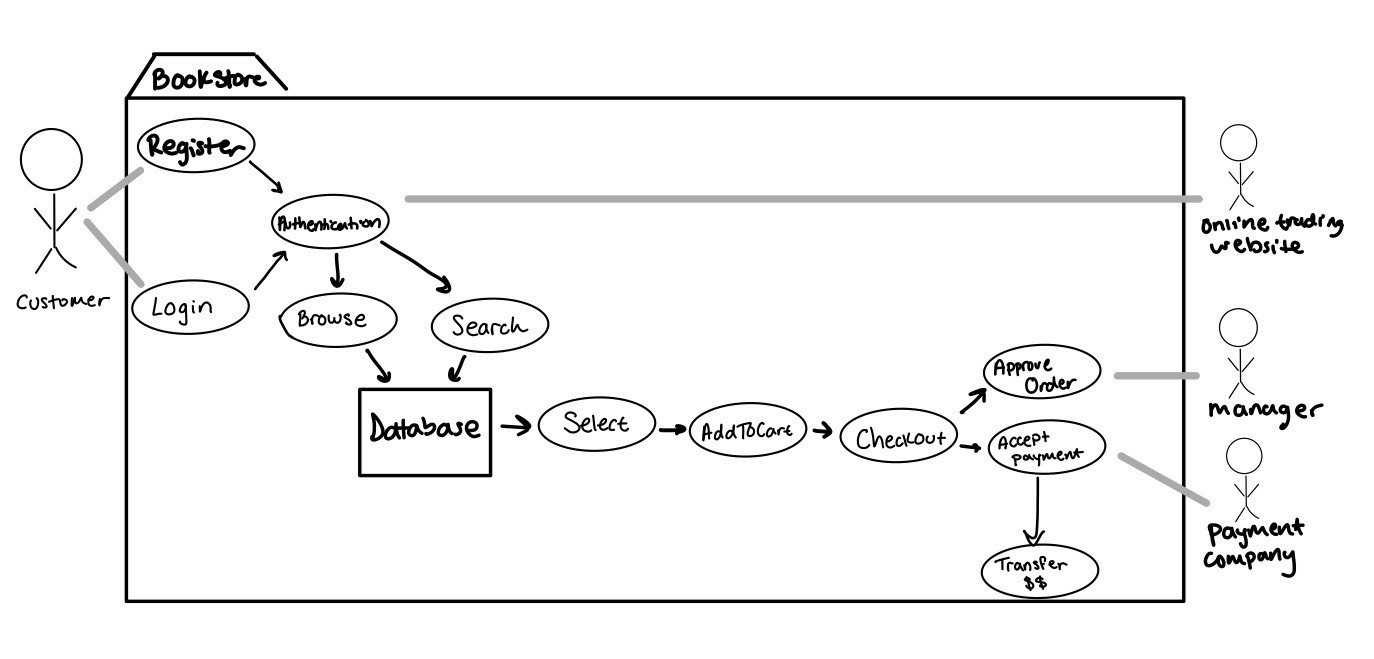
\includegraphics{Figures/bookstore/usecase.jpg}}
    \caption{\label{Figure::bookstoreUseCase} A use-case diagram for the e-Bookstore system that supports the list of functions shown above.}
    \end{figure}

    \begin{figure}
        \centering
        \scalebox{0.8}{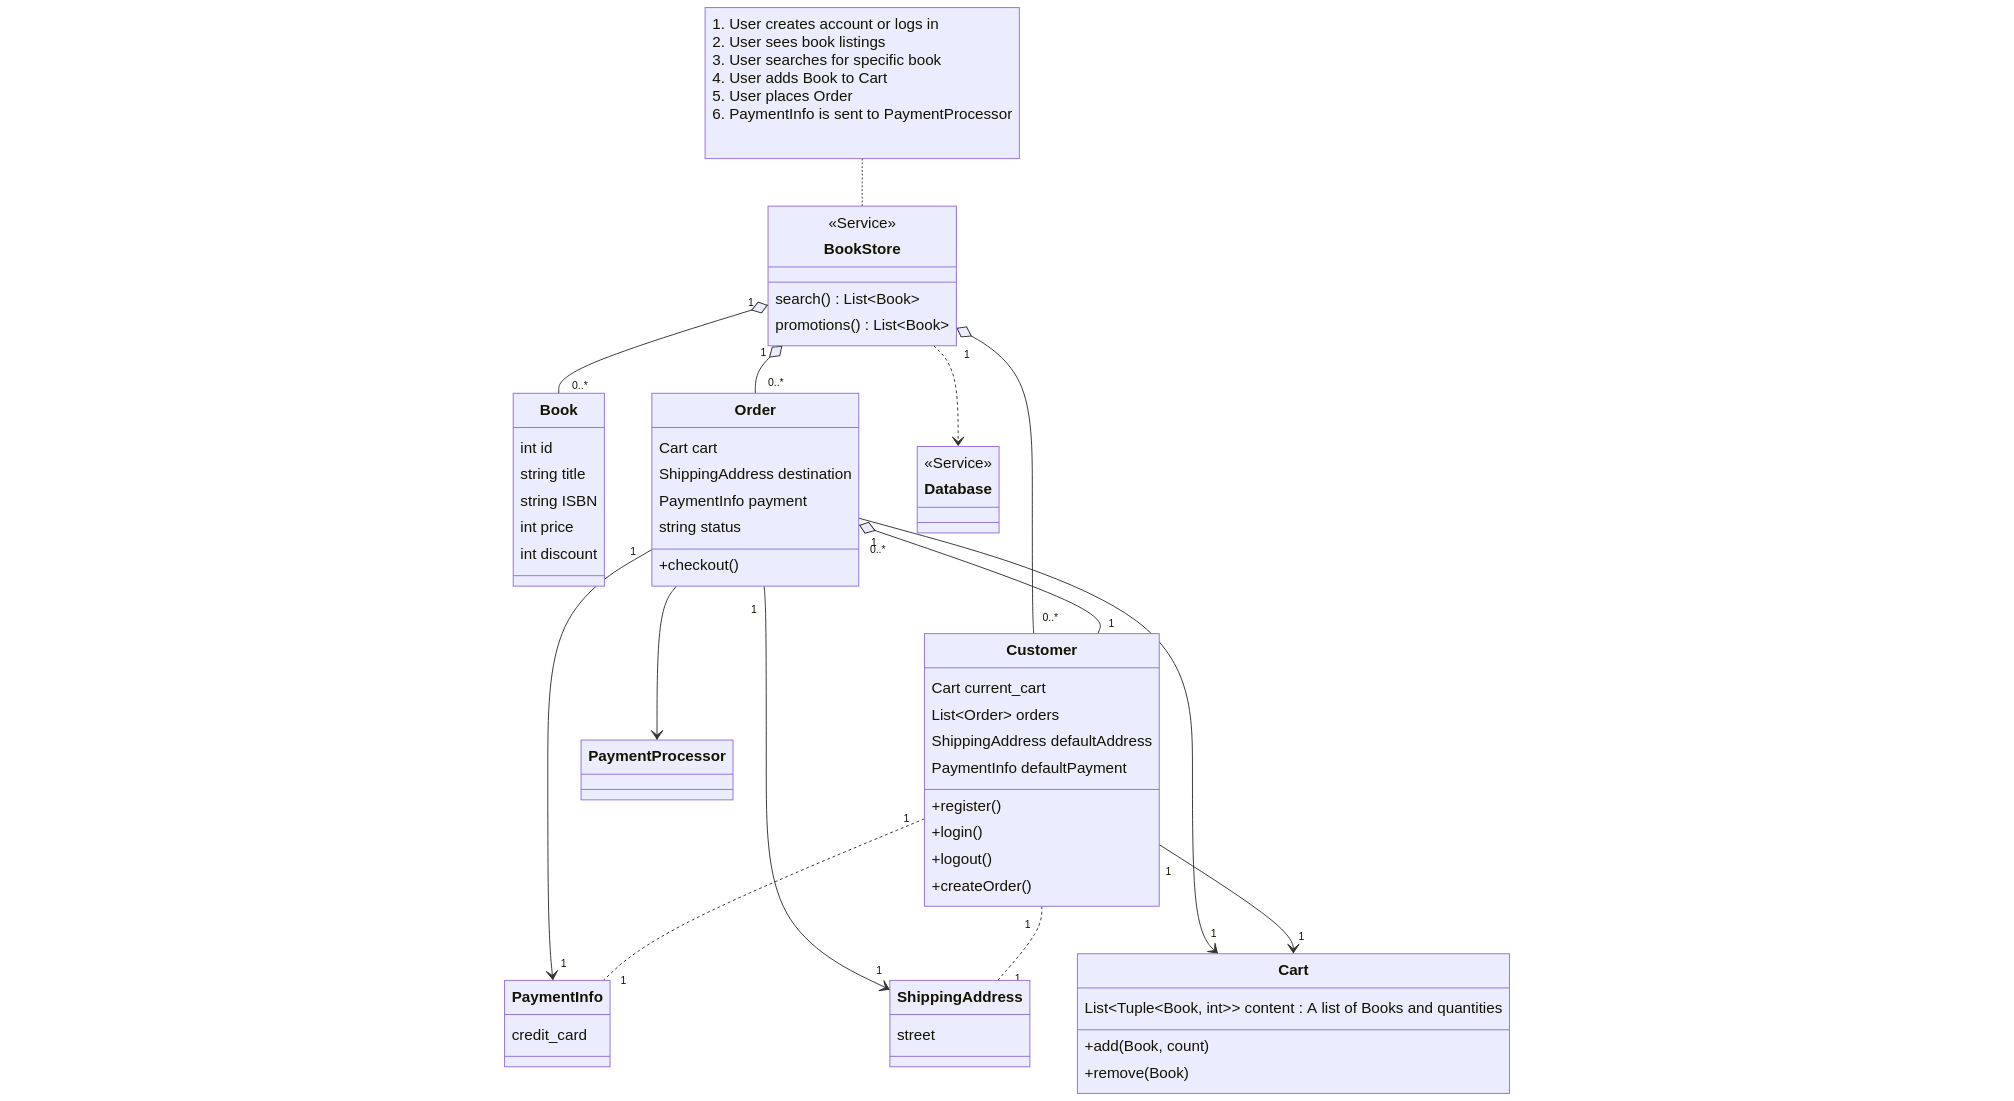
\includegraphics{Figures/bookstore/uml.png}}
        \caption{\label{Figure::bookstoreUML} A class diagram for the e-Bookstore system that illustrates the choices of the main classes and 
        appropriate relationships among them.}
        \end{figure}
\bibliography{bibfile}
%\bibliographystyle{unsrt}
\bibliographystyle{IEEEtran}

%% Initial version by Darian Muresan, Ph.D.
% Edit and adjust as needed.

\documentclass[12pt]{cornell}

% add index support
\makeindex

% graphing programs
\usepackage{color}
\usepackage{psfrag}
\usepackage{verbatim}
\usepackage{fancyhdr}
%\usepackage{titlesec}
\usepackage{fancyvrb}
% hyperlink programs
\usepackage[pdfmark,
breaklinks=true,
colorlinks=true,
citecolor=blue,
linkcolor=blue,
menucolor=black,
pagecolor=black,
urlcolor=blue
]{hyperref} % links in pdf
%\usepackage[colorlinks]{hyperref} % links in dvi
\usepackage{listings}
\usepackage{amsfonts}
\usepackage{amssymb}
%\usepackage{tabto}

\usepackage{tabularx,colortbl}
\usepackage[chapter]{algorithm}
\usepackage{algorithmic}
\usepackage{blindtext}
\usepackage{imakeidx}


\definecolor{DarkGreen}{rgb}{0,0.6,0}
\definecolor{mygreen}{rgb}{0,0.6,0}
\definecolor{mygray}{rgb}{0.5,0.5,0.5}
\definecolor{mymauve}{rgb}{0.58,0,0.82}

\usepackage{tocloft}
\usepackage{amsmath}
\usepackage{tcolorbox}
\usepackage{enumitem}
\usepackage{longtable}
%\usepackage{textcomp}
\usepackage{txfonts}

%part for \part titles
%chap for \chapter titles
%sec for \section titles
%subsec for \subsection titles
%subsubsec for \subsubsection titles
%para for \paragraph titles
%subpara for \subparagraph titles
%fig for figure \caption titles
%subfig for subfigure \caption titles
%tab for table \caption titles
%subtab for subtable \caption titles

% update chapter number spacing
\setlength{\cftchapnumwidth}{2em}
\setlength{\cftsecnumwidth}{2.5em}
\setlength{\cftsubsecnumwidth}{3.5em}
\setlength{\cftsubsubsecnumwidth}{4.5em}

\addtolength{\cftsecindent}{0.5em}
\addtolength{\cftsubsecindent}{0.5em}
\addtolength{\cftsubsubsecindent}{0.5em}

%\titlespacing*{\chapter}{0pt}{-50pt}{20pt}
%\titleformat{\chapter}[display]{\normalfont\huge\bfseries}{\chaptertitlename\
%\thechapter}{20pt}{\Huge}
%\pagestyle{fancy}
%\pagestyle{cornell}
%
%\rhead{F054-021-0172}
%\chead{Nonlinear Enhancement of Visual Target Detection (AF05-T021)}
%\lhead{GSTI}
%\lfoot{\scriptsize Use or disclosure of data on this page is subject
%to the restriction on the title page of this proposal.}
%\cfoot{}
%\rfoot{\thepage}

\newfont{\Bp}{msbm10}
\newfont{\BpBig}{msbm10 scaled\magstep2}
\newfont{\Sc}{eusm10}
\newfont{\ScBig}{eusm10 scaled\magstep3}
\newfont{\Fr}{eufm10}
\newfont{\FrBig}{eufm10 scaled\magstep1}

% some commands:
\newcommand{\dxi}{{\tt m\_xDeltaInput}}
\newcommand{\dyi}{{\tt m\_yDeltaInput}}
\newcommand{\dci}{{\tt m\_cDeltaInput}}
\newcommand{\dxo}{{\tt m\_xDeltaOutput}}
\newcommand{\dyo}{{\tt m\_yDeltaOutput}}
\newcommand{\dco}{{\tt m\_cDeltaOutput}}
\newcommand{\ttf}[1]{{\tt #1}}
\newcommand{\tbl}[2]{{\begin{tabular}{c} #1 \\ #2 \end{tabular}}}

\newcommand{\urltwo}[2]{\mbox{\href{#1}{\tt #2}}}
\newcommand{\qnorm}[1]{\|#1\|_{\bQ}}
\newcommand{\qdot}[2]{\lrb #1, #2 \rrb_{\bQ}}
\newcommand{\kdot}[2]{\lrb #1, #2 \rrb_{\bf k}}
\newcommand{\tdot}[2]{\lrb #1, #2 \rrb}
\newcommand{\mydiff}[2]{\lrb #1 - #2 \rrb}
\newcommand{\lena}{\textit{lena}}
\newcommand{\barb}{\textit{barbara}}
\newcommand{\boat}{\textit{boat}}
\newcommand{\leaves}{\textit{leaves}}
\newcommand{\rings}{\textit{rings}}
\newcommand{\treg}{\textit{train region}}
\newcommand{\dreg}{\textit{denoise region}}
\newcommand{\oreg}{\textit{overlap region}}
\newcommand{\sil}{\sigma_l^2}
\newcommand{\sn}{\sigma^2}
\newcommand{\bn}{{\mbox{\bf \FrBig N}}}
\newcommand{\n}{\mbox{\Fr N}}
%\newcommand{\bn}{\bf N}
%\newcommand{\n}{N}
\newcommand{\bY}{\textbf{Y}}
\newcommand{\bX}{\textbf{X}}
\newcommand{\bb}{\textbf{b}}
\newcommand{\bu}{\textbf{u}}
\newcommand{\bv}{\textbf{v}}
\newcommand{\by}{\textbf{y}}
\newcommand{\bx}{\textbf{x}}
\newcommand{\be}{\textbf{e}}
\newcommand{\bz}{\textbf{z}}
\newcommand{\bs}{\textbf{s}}
\newcommand{\bw}{\textbf{w}}
\newcommand{\bQ}{\textbf{Q}}
\newcommand{\bphi}{\textbf{$\phi$}}
\newcommand{\lsb}{\left[}
\newcommand{\rsb}{\right]}
\newcommand{\lrb}{\left(}
\newcommand{\rrb}{\right)}
\newcommand{\lcb}{\left\{}
\newcommand{\rcb}{\right\}}
\newcommand{\R}{\mbox{\BpBig R}}
\newcommand{\F}{{\cal F}}
\newcommand{\Fk}{\mbox{\Sc F}}
\newcommand{\bQF}{\textbf{Q}_{\mbox{\Sc F}}}
\newcommand{\N}{{\cal N}}
\newcommand{\xlz}{X_l(z)}
\newcommand{\xhz}{X_h(z)}
\newcommand{\xz}{X(z)}
\newcommand{\pr}{ perfect reconstruction }
\newcommand{\smb}{Smith-Barnwell }
\newcommand{\xw}{X(e^{j\omega})}
\newcommand{\xmw}{X(-e^{j\omega})}
\newcommand{\dw}{D(e^{j\omega})}
\newcommand{\dmw}{D(-e^{j\omega})}
\newcommand{\ew}{E(e^{j\omega})}
\newcommand{\emw}{E(-e^{j\omega})}
\newcommand{\fw}{F_0(e^{j\omega})}
\newcommand{\fmw}{F_0(-e^{j\omega})}
\newcommand{\hoz}{H_1(z)}
\newcommand{\hzz}{H_0(z)}
\newcommand{\goz}{G_1(z)}
\newcommand{\gzz}{G_0(z)}
\newcommand{\hzw}{H_{0}(e^{j\omega})}
\newcommand{\hzmw}{H_{0}(-e^{j\omega})}
\newcommand{\hzcw}{H_{0}(e^{-j\omega})}
\newcommand{\how}{H_1(e^{j\omega})}
\newcommand{\homw}{H_1(-e^{j\omega})}
\newcommand{\gzw}{G_0(e^{j\omega})}
\newcommand{\gzmw}{G_0(-e^{j\omega})}
\newcommand{\gow}{G_1(e^{j\omega})}
\newcommand{\gomw}{G_1(-e^{j\omega})}
\newcommand{\wl}{e^{-jwL}}
\newcommand{\aqua}{\textit{AQua with OR }}
\newtheorem{theorem}{Theorem}
\newtheorem{lemma}{Lemma}
\newtheorem{corollary}{Corollary}
\newtheorem{claim}{Claim}
\newtheorem{definition}{Definition}
\newenvironment{proof}{\noindent{\em Proof.}}{\ \hfill Q.E.D.}
%\newtheorem{moduleCount}{L}
\newcommand*{\labelfile}[1]{%
  \label{file:#1}%
}

\lstset{ %
  backgroundcolor=\color{white},   % choose the background color; you must add \usepackage{color} or \usepackage{xcolor}
  basicstyle=\footnotesize,        % the size of the fonts that are used for the code
  breakatwhitespace=false,         % sets if automatic breaks should only happen at whitespace
  breaklines=true,                 % sets automatic line breaking
  captionpos=b,                    % sets the caption-position to bottom
  commentstyle=\color{DarkGreen},    % comment style
  deletekeywords={...},            % if you want to delete keywords from the given language
  escapeinside={\%*}{*)},          % if you want to add LaTeX within your code
  extendedchars=true,              % lets you use non-ASCII characters; for 8-bits encodings only, does not work with UTF-8
  %frame=single,                   % adds a frame around the code
  keepspaces=true,                 % keeps spaces in text, useful for keeping indentation of code (possibly needs columns=flexible)
  keywordstyle=\color{blue},       % keyword style
  language=C++,                    % the language of the code
  morekeywords={*,...},            % if you want to add more keywords to the set
  numbers=left,                    % where to put the line-numbers; possible values are (none, left, right)
  numbersep=5pt,                   % how far the line-numbers are from the code
  numberstyle=\tiny\color{mygray}, % the style that is used for the line-numbers
  rulecolor=\color{black},         % if not set, the frame-color may be changed on line-breaks within not-black text (e.g. comments (green here))
  showspaces=false,                % show spaces everywhere adding particular underscores; it overrides 'showstringspaces'
  showstringspaces=false,          % underline spaces within strings only
  showtabs=false,                  % show tabs within strings adding particular underscores
  stepnumber=1,                    % the step between two line-numbers. If it's 1, each line will be numbered
  stringstyle=\color{mymauve}     % string literal style
  %tabsize=2,                      % sets default tabsize to 2 spaces
  %caption=\lstname                % show the filename of files included with \lstinputlisting; also try caption instead of title
}

% Uncomment draftcopy to get the word DRAFT boldly across the first page
%   By the way, xdvi won't show it but it will come out when you print
%\usepackage[light,all]{draftcopy}		% DRAFT on first page
%\draftcopySetGrey{.97}
%\draftcopyName{Confidential}{150}
%\draftcopFirstPage{1}

% Uncomment drafthead to get the date and DRAFT in the header of pages
% that are normallly numbered on the top, pages 2-n of each chapter for example
% This doesn't work with centered page numbers: \pagestyle{cornellc}
%\usepackage{drafthead}

% Including selective chapters:
% use this to selectively process chapters, etc.  Put a % in front of
% the sections that you don't want done this time.  Includes are
% used instead of \input so that LaTeX will keep track of chapters and
% pages without processing everything.  Don't let any spaces creep in
% around the words or it will not work!


\includeonly{
prologue,
manIntroduction,
manLabOne
}

\makeindex

\begin{document}

\pagenumbering{roman}
\singlespacing
% File: prologue.tex
% Thesis prologue:  Title page, acknowledgements, table of contents,
% list of figures, and list of tables.
%
% this file is to be \include'd after the \begin{document}

% Cornell-style title page
\begin{titlepage}
        \title{Project Title}
        \author{Author(s) Name \\ Stevens.edu }
        \conferraldate{}{\today} \maketitle
\end{titlepage}

% Copyright page
%\begin{copyrightpage}
\makecopyright
%\end{copyrightpage}

% Abstract: the abstract body is pulled from the file abstract.tex;
%  the title is pulled from the \title command in the titlepage section
\begin{abstract}
        %\makeabstitle
        \input abstract      % puts the abstract file here
\end{abstract}

% Biographical information pulled from file bio.tex
%\begin{biosketch} \input bio \end{biosketch}

% Dedication (optional):  pulls information from file dedication.tex
%\begin{dedication} 
%\input dedicate 
%\end{dedication}

% Acknowledgements:  pulls information from file acknow
%\begin{acknowledgements} \input acknow \end{acknowledgements}

% Table of contents
\contentspage

% If you have no tables or figures put a % in front of the list page line
% List of tables
\tablelistpage

% List of figures
\figurelistpage



\setcounter{page}{1}        % set page counter
\pagenumbering{arabic}      % set page number style
\pagestyle{fancy}         % top right page numbers
%\pagestyle{cornell}
%\pagestyle{cornellc}       % centered page numbers, disables drafthead

\renewcommand{\chaptermark}[1]{\markboth{#1}{}}
\renewcommand{\sectionmark}[1]{\markright{#1}{}}

\fancyhead{} % clear all fields

\lhead{Chapter \thechapter}
%\lhead{\thechapter}
\chead{\leftmark}
\rhead{\thepage}


\lfoot{Chapter \thechapter}
\cfoot{\copyright Stevens -- \today \mbox{} -- Project Name}
\rfoot{\thepage}

\renewcommand{\headrulewidth}{0.4pt}
\renewcommand{\footrulewidth}{0.4pt}

%\rhead{F054-021-0172}
%\chead{Nonlinear Enhancement of Visual Target Detection (AF05-T021)}
%\lhead{GSTI}
%\lfoot{\scriptsize Use or disclosure of data on this page is subject
%to the restriction on the title page of this proposal.}
%\cfoot{}
%\rfoot{\thepage}


\singlespacing
\chapter{Introduction \\
  \small{\textit{-- Author Name}}
  \index{Chapter!introduction}
  \index{introduction}
  \label{Chapter::Introduction}}

% Add a section and label it so that we can reference it later
\section{Team Introduction \label{Section::TeamIntroduction}}

\subsection{Carson McManus}

I'm Carson McManus and I'm a 4/5 undergrad Software Engineer. I've written a lot of code over the past 13 years, and I maintain and contribute to open source projects. Programming is something that gives me a lot of joy, and I'm always honing my craft.

\subsection{Sophia DiCuffa}

My name is Sophia DiCuffa and I am a 3/4 Software Engineer! I've been coding for four years and I am always excited to learn new things.
\chapter{Bookstore UML Modeling \\
  \small{\textit{-- Evan Ciok, Sophia DiCuffa, Carson McManus}}
  \index{Chapter!labone}
  \index{Lab One}
  \label{Chapter::LabOne}}

% Add a section and label it so that we can reference it later
\section{Bookstore UML Modeling \label{Section::LabOne}}

\begin{figure}
    \centering
    \scalebox{0.8}{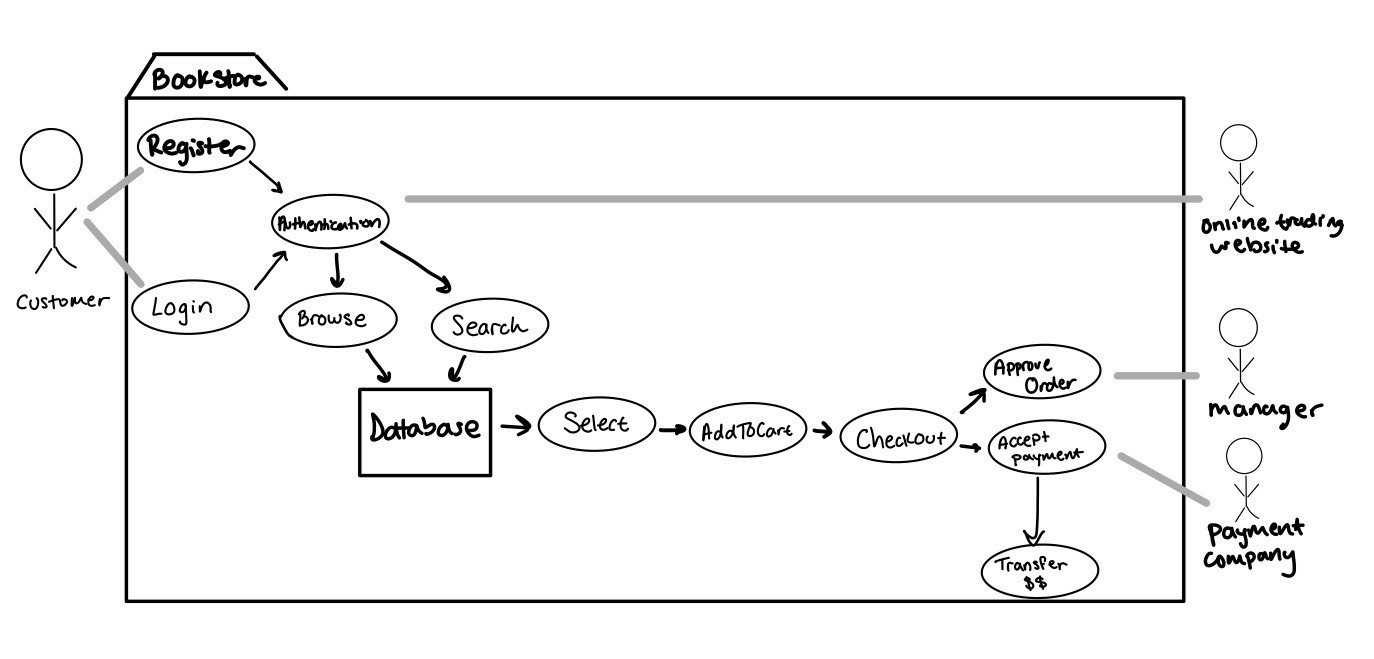
\includegraphics{Figures/bookstore/usecase.jpg}}
    \caption{\label{Figure::bookstoreUseCase} A use-case diagram for the e-Bookstore system that supports the list of functions shown above.}
    \end{figure}

    \begin{figure}
        \centering
        \scalebox{0.8}{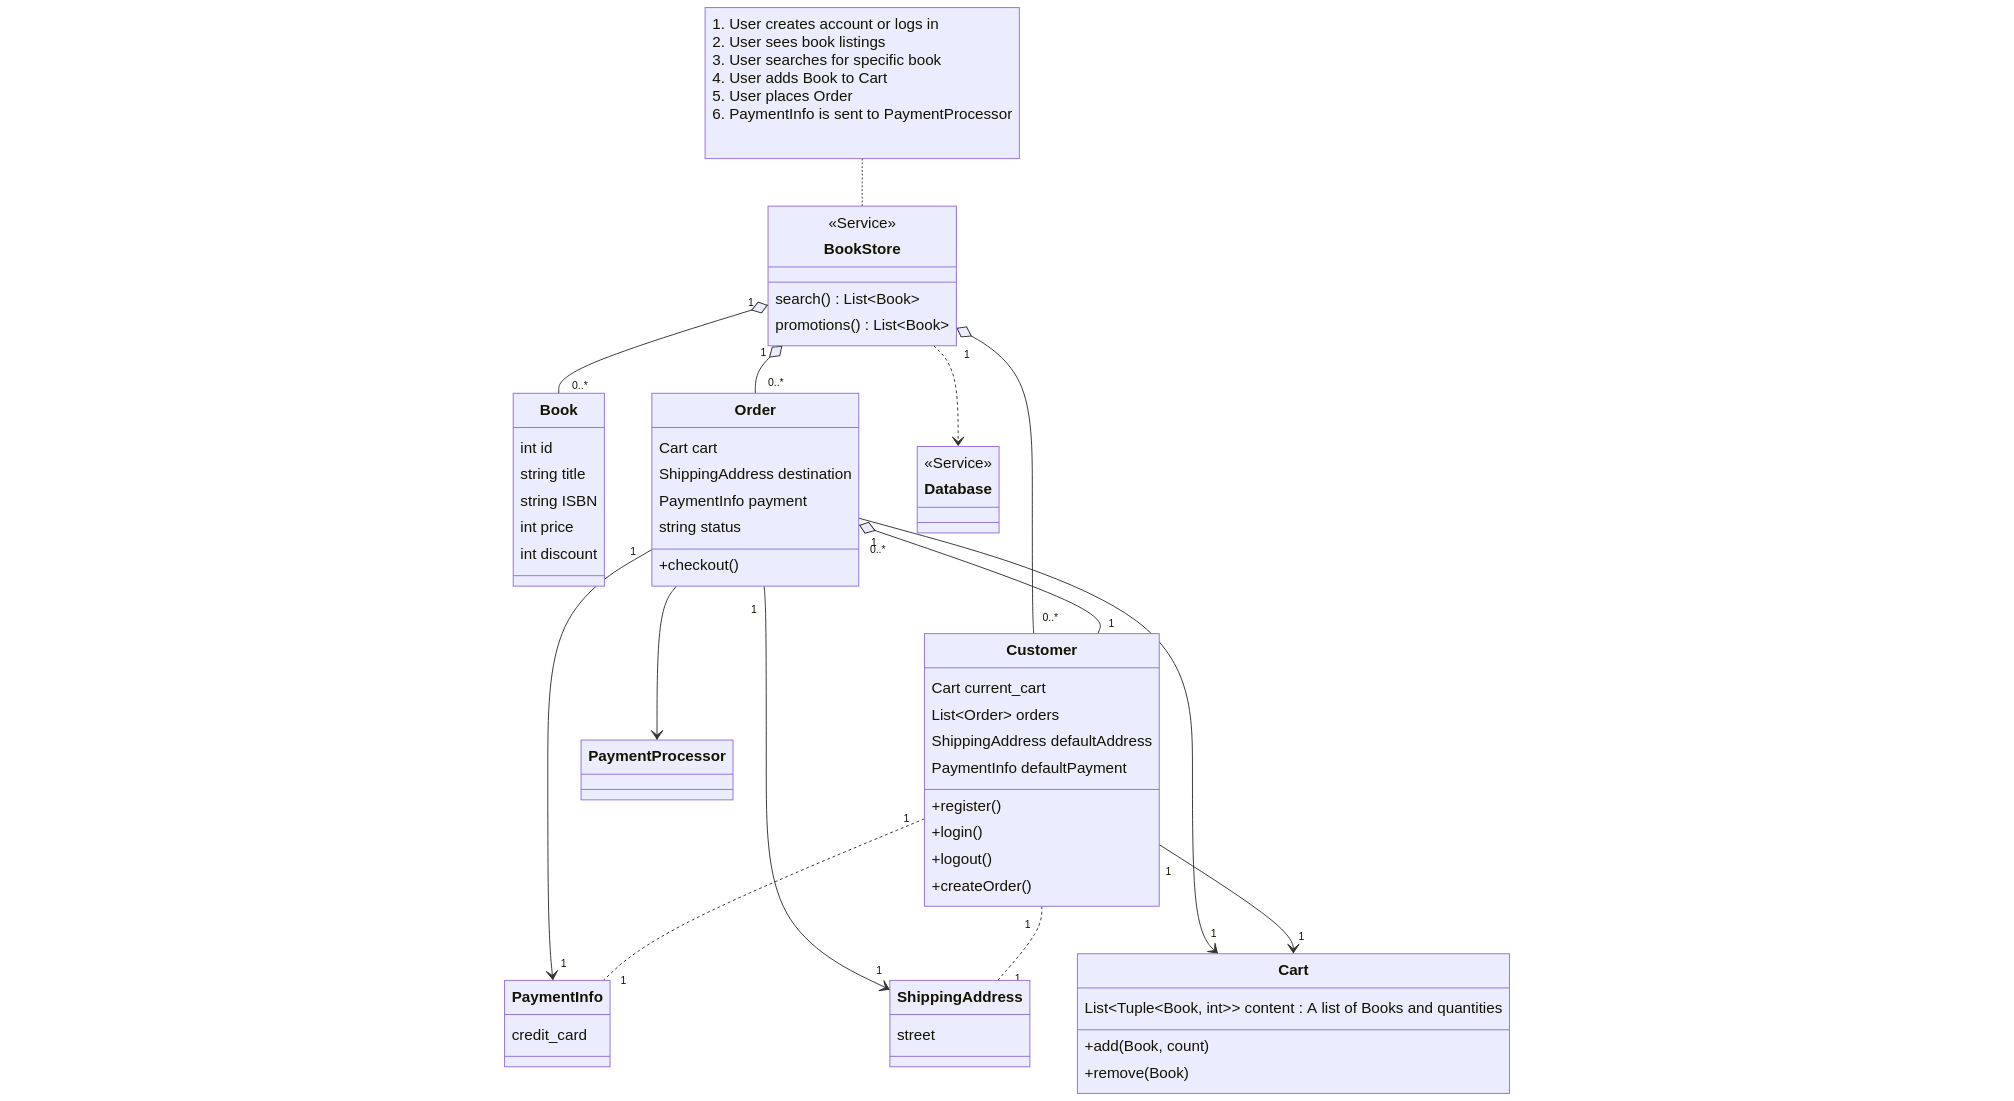
\includegraphics{Figures/bookstore/uml.png}}
        \caption{\label{Figure::bookstoreUML} A class diagram for the e-Bookstore system that illustrates the choices of the main classes and 
        appropriate relationships among them.}
        \end{figure}
\bibliography{bibfile}
%\bibliographystyle{unsrt}
\bibliographystyle{IEEEtran}

%% Initial version by Darian Muresan, Ph.D.
% Edit and adjust as needed.

\documentclass[12pt]{cornell}

% add index support
\makeindex

% graphing programs
\usepackage{color}
\usepackage{psfrag}
\usepackage{verbatim}
\usepackage{fancyhdr}
%\usepackage{titlesec}
\usepackage{fancyvrb}
% hyperlink programs
\usepackage[pdfmark,
breaklinks=true,
colorlinks=true,
citecolor=blue,
linkcolor=blue,
menucolor=black,
pagecolor=black,
urlcolor=blue
]{hyperref} % links in pdf
%\usepackage[colorlinks]{hyperref} % links in dvi
\usepackage{listings}
\usepackage{amsfonts}
\usepackage{amssymb}
%\usepackage{tabto}

\usepackage{tabularx,colortbl}
\usepackage[chapter]{algorithm}
\usepackage{algorithmic}
\usepackage{blindtext}
\usepackage{imakeidx}


\definecolor{DarkGreen}{rgb}{0,0.6,0}
\definecolor{mygreen}{rgb}{0,0.6,0}
\definecolor{mygray}{rgb}{0.5,0.5,0.5}
\definecolor{mymauve}{rgb}{0.58,0,0.82}

\usepackage{tocloft}
\usepackage{amsmath}
\usepackage{tcolorbox}
\usepackage{enumitem}
\usepackage{longtable}
%\usepackage{textcomp}
\usepackage{txfonts}

%part for \part titles
%chap for \chapter titles
%sec for \section titles
%subsec for \subsection titles
%subsubsec for \subsubsection titles
%para for \paragraph titles
%subpara for \subparagraph titles
%fig for figure \caption titles
%subfig for subfigure \caption titles
%tab for table \caption titles
%subtab for subtable \caption titles

% update chapter number spacing
\setlength{\cftchapnumwidth}{2em}
\setlength{\cftsecnumwidth}{2.5em}
\setlength{\cftsubsecnumwidth}{3.5em}
\setlength{\cftsubsubsecnumwidth}{4.5em}

\addtolength{\cftsecindent}{0.5em}
\addtolength{\cftsubsecindent}{0.5em}
\addtolength{\cftsubsubsecindent}{0.5em}

%\titlespacing*{\chapter}{0pt}{-50pt}{20pt}
%\titleformat{\chapter}[display]{\normalfont\huge\bfseries}{\chaptertitlename\
%\thechapter}{20pt}{\Huge}
%\pagestyle{fancy}
%\pagestyle{cornell}
%
%\rhead{F054-021-0172}
%\chead{Nonlinear Enhancement of Visual Target Detection (AF05-T021)}
%\lhead{GSTI}
%\lfoot{\scriptsize Use or disclosure of data on this page is subject
%to the restriction on the title page of this proposal.}
%\cfoot{}
%\rfoot{\thepage}

\newfont{\Bp}{msbm10}
\newfont{\BpBig}{msbm10 scaled\magstep2}
\newfont{\Sc}{eusm10}
\newfont{\ScBig}{eusm10 scaled\magstep3}
\newfont{\Fr}{eufm10}
\newfont{\FrBig}{eufm10 scaled\magstep1}

% some commands:
\newcommand{\dxi}{{\tt m\_xDeltaInput}}
\newcommand{\dyi}{{\tt m\_yDeltaInput}}
\newcommand{\dci}{{\tt m\_cDeltaInput}}
\newcommand{\dxo}{{\tt m\_xDeltaOutput}}
\newcommand{\dyo}{{\tt m\_yDeltaOutput}}
\newcommand{\dco}{{\tt m\_cDeltaOutput}}
\newcommand{\ttf}[1]{{\tt #1}}
\newcommand{\tbl}[2]{{\begin{tabular}{c} #1 \\ #2 \end{tabular}}}

\newcommand{\urltwo}[2]{\mbox{\href{#1}{\tt #2}}}
\newcommand{\qnorm}[1]{\|#1\|_{\bQ}}
\newcommand{\qdot}[2]{\lrb #1, #2 \rrb_{\bQ}}
\newcommand{\kdot}[2]{\lrb #1, #2 \rrb_{\bf k}}
\newcommand{\tdot}[2]{\lrb #1, #2 \rrb}
\newcommand{\mydiff}[2]{\lrb #1 - #2 \rrb}
\newcommand{\lena}{\textit{lena}}
\newcommand{\barb}{\textit{barbara}}
\newcommand{\boat}{\textit{boat}}
\newcommand{\leaves}{\textit{leaves}}
\newcommand{\rings}{\textit{rings}}
\newcommand{\treg}{\textit{train region}}
\newcommand{\dreg}{\textit{denoise region}}
\newcommand{\oreg}{\textit{overlap region}}
\newcommand{\sil}{\sigma_l^2}
\newcommand{\sn}{\sigma^2}
\newcommand{\bn}{{\mbox{\bf \FrBig N}}}
\newcommand{\n}{\mbox{\Fr N}}
%\newcommand{\bn}{\bf N}
%\newcommand{\n}{N}
\newcommand{\bY}{\textbf{Y}}
\newcommand{\bX}{\textbf{X}}
\newcommand{\bb}{\textbf{b}}
\newcommand{\bu}{\textbf{u}}
\newcommand{\bv}{\textbf{v}}
\newcommand{\by}{\textbf{y}}
\newcommand{\bx}{\textbf{x}}
\newcommand{\be}{\textbf{e}}
\newcommand{\bz}{\textbf{z}}
\newcommand{\bs}{\textbf{s}}
\newcommand{\bw}{\textbf{w}}
\newcommand{\bQ}{\textbf{Q}}
\newcommand{\bphi}{\textbf{$\phi$}}
\newcommand{\lsb}{\left[}
\newcommand{\rsb}{\right]}
\newcommand{\lrb}{\left(}
\newcommand{\rrb}{\right)}
\newcommand{\lcb}{\left\{}
\newcommand{\rcb}{\right\}}
\newcommand{\R}{\mbox{\BpBig R}}
\newcommand{\F}{{\cal F}}
\newcommand{\Fk}{\mbox{\Sc F}}
\newcommand{\bQF}{\textbf{Q}_{\mbox{\Sc F}}}
\newcommand{\N}{{\cal N}}
\newcommand{\xlz}{X_l(z)}
\newcommand{\xhz}{X_h(z)}
\newcommand{\xz}{X(z)}
\newcommand{\pr}{ perfect reconstruction }
\newcommand{\smb}{Smith-Barnwell }
\newcommand{\xw}{X(e^{j\omega})}
\newcommand{\xmw}{X(-e^{j\omega})}
\newcommand{\dw}{D(e^{j\omega})}
\newcommand{\dmw}{D(-e^{j\omega})}
\newcommand{\ew}{E(e^{j\omega})}
\newcommand{\emw}{E(-e^{j\omega})}
\newcommand{\fw}{F_0(e^{j\omega})}
\newcommand{\fmw}{F_0(-e^{j\omega})}
\newcommand{\hoz}{H_1(z)}
\newcommand{\hzz}{H_0(z)}
\newcommand{\goz}{G_1(z)}
\newcommand{\gzz}{G_0(z)}
\newcommand{\hzw}{H_{0}(e^{j\omega})}
\newcommand{\hzmw}{H_{0}(-e^{j\omega})}
\newcommand{\hzcw}{H_{0}(e^{-j\omega})}
\newcommand{\how}{H_1(e^{j\omega})}
\newcommand{\homw}{H_1(-e^{j\omega})}
\newcommand{\gzw}{G_0(e^{j\omega})}
\newcommand{\gzmw}{G_0(-e^{j\omega})}
\newcommand{\gow}{G_1(e^{j\omega})}
\newcommand{\gomw}{G_1(-e^{j\omega})}
\newcommand{\wl}{e^{-jwL}}
\newcommand{\aqua}{\textit{AQua with OR }}
\newtheorem{theorem}{Theorem}
\newtheorem{lemma}{Lemma}
\newtheorem{corollary}{Corollary}
\newtheorem{claim}{Claim}
\newtheorem{definition}{Definition}
\newenvironment{proof}{\noindent{\em Proof.}}{\ \hfill Q.E.D.}
%\newtheorem{moduleCount}{L}
\newcommand*{\labelfile}[1]{%
  \label{file:#1}%
}

\lstset{ %
  backgroundcolor=\color{white},   % choose the background color; you must add \usepackage{color} or \usepackage{xcolor}
  basicstyle=\footnotesize,        % the size of the fonts that are used for the code
  breakatwhitespace=false,         % sets if automatic breaks should only happen at whitespace
  breaklines=true,                 % sets automatic line breaking
  captionpos=b,                    % sets the caption-position to bottom
  commentstyle=\color{DarkGreen},    % comment style
  deletekeywords={...},            % if you want to delete keywords from the given language
  escapeinside={\%*}{*)},          % if you want to add LaTeX within your code
  extendedchars=true,              % lets you use non-ASCII characters; for 8-bits encodings only, does not work with UTF-8
  %frame=single,                   % adds a frame around the code
  keepspaces=true,                 % keeps spaces in text, useful for keeping indentation of code (possibly needs columns=flexible)
  keywordstyle=\color{blue},       % keyword style
  language=C++,                    % the language of the code
  morekeywords={*,...},            % if you want to add more keywords to the set
  numbers=left,                    % where to put the line-numbers; possible values are (none, left, right)
  numbersep=5pt,                   % how far the line-numbers are from the code
  numberstyle=\tiny\color{mygray}, % the style that is used for the line-numbers
  rulecolor=\color{black},         % if not set, the frame-color may be changed on line-breaks within not-black text (e.g. comments (green here))
  showspaces=false,                % show spaces everywhere adding particular underscores; it overrides 'showstringspaces'
  showstringspaces=false,          % underline spaces within strings only
  showtabs=false,                  % show tabs within strings adding particular underscores
  stepnumber=1,                    % the step between two line-numbers. If it's 1, each line will be numbered
  stringstyle=\color{mymauve}     % string literal style
  %tabsize=2,                      % sets default tabsize to 2 spaces
  %caption=\lstname                % show the filename of files included with \lstinputlisting; also try caption instead of title
}

% Uncomment draftcopy to get the word DRAFT boldly across the first page
%   By the way, xdvi won't show it but it will come out when you print
%\usepackage[light,all]{draftcopy}		% DRAFT on first page
%\draftcopySetGrey{.97}
%\draftcopyName{Confidential}{150}
%\draftcopFirstPage{1}

% Uncomment drafthead to get the date and DRAFT in the header of pages
% that are normallly numbered on the top, pages 2-n of each chapter for example
% This doesn't work with centered page numbers: \pagestyle{cornellc}
%\usepackage{drafthead}

% Including selective chapters:
% use this to selectively process chapters, etc.  Put a % in front of
% the sections that you don't want done this time.  Includes are
% used instead of \input so that LaTeX will keep track of chapters and
% pages without processing everything.  Don't let any spaces creep in
% around the words or it will not work!


\includeonly{
prologue,
manIntroduction,
manLabOne
}

\makeindex

\begin{document}

\pagenumbering{roman}
\singlespacing
\include{prologue}

\setcounter{page}{1}        % set page counter
\pagenumbering{arabic}      % set page number style
\pagestyle{fancy}         % top right page numbers
%\pagestyle{cornell}
%\pagestyle{cornellc}       % centered page numbers, disables drafthead

\renewcommand{\chaptermark}[1]{\markboth{#1}{}}
\renewcommand{\sectionmark}[1]{\markright{#1}{}}

\fancyhead{} % clear all fields

\lhead{Chapter \thechapter}
%\lhead{\thechapter}
\chead{\leftmark}
\rhead{\thepage}


\lfoot{Chapter \thechapter}
\cfoot{\copyright Stevens -- \today \mbox{} -- Project Name}
\rfoot{\thepage}

\renewcommand{\headrulewidth}{0.4pt}
\renewcommand{\footrulewidth}{0.4pt}

%\rhead{F054-021-0172}
%\chead{Nonlinear Enhancement of Visual Target Detection (AF05-T021)}
%\lhead{GSTI}
%\lfoot{\scriptsize Use or disclosure of data on this page is subject
%to the restriction on the title page of this proposal.}
%\cfoot{}
%\rfoot{\thepage}


\singlespacing
\include{manIntroduction}
\include{manLabOne}
\bibliography{bibfile}
%\bibliographystyle{unsrt}
\bibliographystyle{IEEEtran}

%\input{manual.ind}
\printindex
\end{document}

\printindex
\end{document}

\printindex
\end{document}

\printindex
\end{document}
